\subsection{The Cauchy--Goursat Theorem}
It is important to know the differential 2-forms even for a single variable complex function. Consider \(z=x+\ii y\) and \(\overline{z}=x-\ii y\). We can then define their corresponding differentials:
\[\ddz=\ddx+\ii\ddy,\quad\dd{\overline{z}}=\ddx-\ii\ddy.\]
The antisymmetric properties of differential forms still hold in complex space. By taking the wedge product of the two basis complex differential forms, we get
\begin{align*}
    \dd{\overline{z}}\wedge\ddz & =\paren{\ddx-\ii\ddy}\wedge\paren{\ddx+\ii\ddy} \\
    & =2\ii\ddx\wedge\ddy.
\end{align*}
Analogous to the real case, a 0-form is defined as a scalar-valued function in the form \(f\paren{z,\overline{z}}\), a 1-form in the form of \(\omega_0\ddz+\omega_1\dd{\overline{z}}\), and a 2-form as \(\omega_0\ddz\wedge\dd{\overline{z}}\). The exterior differential operator for this one-dimensional case is defined as \(\partial+\overline{\partial}\), where \(\partial=\ddz\wedge\pdv{}{z}\) and \(\overline{\partial}=\dd{\overline{z}}\wedge\pdv{}{\overline{z}}\). Occasionally, one will informally use \(\partial\) and \(\overline{\partial}\) as an abbreviation for \(\pdv{z}\) and \(\pdv{\overline{z}}\) respectively.
\begin{theorem}[Lusin Area Theorem]\label{thm:lusinarea}
    For a region \(U\subset\mathbb{C}\) and \(f:U\to\mathbb{C}\) univalent, the area of the image \(f(U)\) is equal to \[\int_{U}\abs{f'(z)}^2\dd{A}.\]
\end{theorem}
\begin{proof}
    We aim to find \[\int_{f(U)}\dd{A}.\]
    By the properties above,
    \begin{align*}
        \int_{f(U)}\dd{u}\wedge\dd{v} & =\frac{\ii}{2}\int_{f(U)}\dd{w}\wedge\dd{\overline{w}}=\frac{\ii}{2}\int_{U}\dd{f(z)}\wedge\dd{\overline{f(z)}} \\
        & =\frac{\ii}{2}\int_{U}{f'(z)\ddz}\wedge{\overline{f'(z)}\dd{\overline{z}}}=\int_U\abs{f'(z)}^2\ddx\wedge\ddy,
    \end{align*}
    as desired.
\end{proof}
\begin{remark}
    The Jacobian determinant of \(u,v\) with respect to \(x,y\), for a holomorphic function \(f(z)=u(x,y)+\ii v(x,y)\) is equal to \[\mqty|u'_x&u'_y\\v'_x&v'_y|=\pdv{u}{x}\pdv{v}{y}-\pdv{u}{y}\pdv{v}{x}=\paren{\pdv{u}{x}}^2+\paren{\pdv{u}{y}}^2=\abs{f'(z)}^2\] by \cref{eq:holomorphicderivativedecomposition}.
\end{remark}
\begin{theorem}[Green's Theorem, Complex Form]\label{thm:complexgreen}
    Let \(U\subset\mathbb{C}\) be bounded with a piecewise smooth boundary \(\partial U\). For two scalar functions \(\omega_1=\omega_1\paren{z,\overline{z}}\) and \(\omega_2=\omega_2\paren{z,\overline{z}}\) satisfying \(\omega_1,\omega_2\in C^1\paren{\overline{U}}\), define the 1-form \(\omega=\omega_1\ddz+\omega_2\dd{\overline{z}}\). Then,
    \begin{equation}
        \int_{\partial U}\omega=\int_U\dd{\omega}.\label{eq:complexgreen}
    \end{equation}
\end{theorem}
\begin{proof}
    For real-valued functions \(\xi_1,\xi_2,\eta_1,\eta_2\), let \[\omega_1=\xi_1+\ii\eta_1\qq{and let}\omega_2=\xi_2+\ii\eta_2.\]
    Then,
    \begin{align}
        \omega & =\paren{\xi_1+\ii\eta_1}\ddz+\paren{\xi_2+\ii\eta_2}\dd{\overline{z}}\label{eq:complexgreen_omegaexpansionintermediate}                                                   \\
        & =\paren{\xi_1+\ii\eta_1}\paren{\ddx+\ii\ddy}+\paren{\xi_2+\ii\eta_2}\paren{\ddx-\ii\ddy}\nonumber                                                                         \\
        & =\xi_1\ddx+\ii\eta_1\ddx+\ii\xi_1\ddy-\eta_1\ddy+\xi_2\ddx+\ii\eta_2\ddx-\ii\xi_2\ddy+\eta_2\ddy\nonumber                                                                 \\
        & =\qty[\paren{\xi_1+\xi_2}\ddx+\paren{\eta_2-\eta_1}\ddy]+\ii\qty[\paren{\eta_1+\eta_2}\ddx+\paren{\xi_1-\xi_2}\ddy]\label{eq:complexgreen_realandcomplexdxdyintermediate}
    \end{align}
    Each of \(\xi_1,\xi_2,\eta_1,\eta_2\) are real-valued functions that can be represented with a domain of \(\mathbb{R}^2\). We then will apply the \(\dd=\partial+\overline{\partial}\) definition of the exterior derivative and relate it to \cref{eq:complexgreen}. Starting with \cref{eq:complexgreen_omegaexpansionintermediate},
    \begin{align}
        \dd{\omega} & =\paren{\partial+\overline{\partial}}\paren{\xi_1+\ii\eta_1}\ddz+\paren{\partial+\overline{\partial}}\paren{\xi_2+\ii\eta_2}\dd{\overline{z}}\nonumber                                                       \\
        & =\paren{\pdv{\xi_1}{\overline{z}}+\ii\pdv{\eta_1}{\overline{z}}}\dd{\overline{z}}\wedge\ddz+\paren{\pdv{\xi_2}{z}+\ii\pdv{\eta_2}{z}}\ddz\wedge\dd{\overline{z}}\nonumber                                    \\
        & =2\paren{\ii\pdv{\xi_1}{\overline{z}}-\pdv{\eta_1}{\overline{z}}-\ii\pdv{\xi_2}{z}+\pdv{\eta_2}{z}}\ddx\wedge\ddy\nonumber                                                                                   \\
        & =\paren{\ii\pdv{\xi_1}{x}-\pdv{\xi_1}{y}-\pdv{\eta_1}{x}-\ii\pdv{\eta_1}{y}-\ii\pdv{\xi_2}{x}-\pdv{\xi_2}{y}+\pdv{\eta_2}{x}-\ii\pdv{\eta_2}{y}}\ddx\wedge\ddy\nonumber                                      \\
        & =\paren{\pdv{\eta_2}{x}-\pdv{\xi_1}{y}-\pdv{\eta_1}{x}-\pdv{\xi_2}{y}}\dd{A}+\ii\paren{\pdv{\xi_1}{x}-\pdv{\eta_1}{y}-\pdv{\xi_2}{x}-\pdv{\eta_2}{y}}\dd{A}.\label{eq:complexgreen_exteriorderivativeresult}
    \end{align}
    From \cref{eq:complexgreen_realandcomplexdxdyintermediate}, we can apply \cref{thm:realgreen}. For the real component of \(\omega\), we obtain
    \[\int_{\partial U}\paren{\xi_1+\xi_2}\ddx+\paren{\eta_2-\eta_1}\ddy=\iint_U\paren{\pdv{\eta_2}{x}-\pdv{\xi_1}{y}-\pdv{\eta_1}{x}-\pdv{\xi_2}{y}}\ddx\ddy,\]
    and for the imaginary component,
    \[\int_{\partial U}\paren{\eta_1+\eta_2}\ddx+\paren{\xi_1-\xi_2}\ddy=\iint_U\paren{\pdv{\xi_1}{x}-\pdv{\eta_1}{y}-\pdv{\xi_2}{x}-\pdv{\eta_2}{y}}\ddx\ddy,\]
    and the integrands on the right side both match those of \cref{eq:complexgreen_exteriorderivativeresult}.
\end{proof}
The theorem above is only a specific case of the Stokes-Cartan Theorem (\cref{thm:stokescartan}). However, it proves the validity of the treatment of the \(\partial\) and \(\overline{\partial}\) operators, and the generalization to forms with basis \(\ddz\) and \(\dd{\overline{z}}\).
\begin{theorem}[\textsc{Cauchy--Pompeiu}]\label{thm:pompeiu}
    Let \(U\subset\mathbb{C}\) be bounded with a piecewise \(C^1\) boundary \(\partial U\). Let \(f(z)\in C^1\qty(\overline{U})\). Then \(\forall z\in U\setminus\partial U\),
    \begin{equation}
        f(z)=\frac{1}{2\uppi\ii}\qty(\int_{\partial U}\frac{f(\zeta)}{\zeta-z}\mathop{\dd{\zeta}}-\int_{U}\pdv{f(\zeta)}{\overline{\zeta}}\frac{\dd{\overline{\zeta}}\wedge\ddzeta}{\zeta-z}).
    \end{equation}
\end{theorem}
\begin{proof}
    Since \(z\in U\setminus\partial U\), \(\exists\varepsilon>0\) such that \(D(z,\varepsilon)\subset U\). Consider the complex differential form \[\frac{f(\zeta)\ddzeta}{\zeta-z}\]
    with a singularity at \(\zeta=z\). Consider the region \(U\setminus D(z,\varepsilon)\). Since \(f\in C^1\paren{\overline{U}}\), by applying Green's Theorem (\cref{thm:complexgreen}),
    \begin{equation}
        \int_{U\setminus D(z,\varepsilon)}\dd(\frac{f(\zeta)\ddzeta}{\zeta-z})=\int_{\partial U}\frac{f(\zeta)\ddzeta}{\zeta-z}-\int_{\partial D(z,\varepsilon)}\frac{f(\zeta)\ddzeta}{\zeta-z}.\label{eq:pompeiu_directintermediate}
    \end{equation}
    By properties of \(\dd\), the expression is equal to
    \begin{align*}
        \int_{U\setminus D(z,\varepsilon)}\qty(\partial+\overline{\partial})\qty(\frac{f(\zeta)}{\zeta-z})\wedge\ddzeta & =\int_{U\setminus D(z,\varepsilon)}\pdv{}{\zeta}\qty(\frac{f(\zeta)}{\zeta-z})\ddzeta\wedge\ddzeta \\
        & \quad+\pdv{\overline{\zeta}}\qty(\frac{f(\zeta)}{\zeta-z})\dd{\overline{\zeta}}\wedge\ddzeta.
    \end{align*}
    The first term in the integrand vanishes as it contains \(\ddzeta\wedge\ddzeta\). The second term can be simplified using the fact that \(\pdv{\overline{\zeta}}(\frac{1}{\zeta-z})=0\), leading to
    \[\int_{U\setminus D(z,\varepsilon)}\pdv{f}{\overline{\zeta}}\cdot\frac{\dd{\overline{\zeta}}\wedge\ddzeta}{\zeta-z}.\]
    The rightmost term in \cref{eq:pompeiu_directintermediate} can be parameterized with \(\zeta=z+\varepsilon\ee^{\ii t}\), \(t\in[0,2\uppi]\). Then,
    \begin{gather*}
        \int_{\partial D(z,\varepsilon)}\frac{f(\zeta)\ddzeta}{\zeta-z}=\int_0^{2\uppi}\frac{f\paren{z+\varepsilon\ee^{\ii t}}}{\varepsilon\ee^{\ii t}}\cdot\ii\varepsilon\ee^{\ii t}\dd{t}=\ii\int_0^{2\uppi}f(z+\varepsilon\ee^{\ii t})\dd{t}\\
        =\ii\int_0^{2\uppi}\qty(f\paren{z+\varepsilon\ee^{\ii t}}-f(z))\dd{t}+\ii\int_0^{2\uppi}f(z)\dd{t}.
    \end{gather*}
    Because \(f\in C^1\qty(\overline{U})\), by \cref{prop:c1lipschitz}, \(f\) is Lipschitz continuous on \(\overline{U}\), and \(\exists M\in\mathbb{R}_{>0}\) such that \(\forall z_0,z_1\in\overline{U}\), \(\abs{f\paren{z_1}-f\paren{z_0}}\le M\abs{z_1-z_0}\). On \(\partial D(z,\varepsilon)\), we get that \(\abs{f(z+\varepsilon\ee^{\ii t})-f(z)}\leq M\varepsilon\). Therefore, \[\abs{\int_0^{2\uppi}\qty(f\qty(z+\varepsilon\ee^{\ii t})-f(z))\dd{t}}\leq\int_0^{2\uppi}\abs{f\qty(z+\varepsilon\ee^{\ii t})-f(z)}\dd{t}\leq 2M\uppi\varepsilon,\] which approaches 0 as \(\varepsilon\to0\). Taking this limit, we obtain
    \begin{equation}
        2\uppi\ii f(z)=\int_{\partial U}\frac{f(\zeta)\ddzeta}{\zeta-z}-\int_{U}\pdv{f}{\overline{\zeta}}\cdot\frac{\dd{\overline{\zeta}}\wedge\ddzeta}{\zeta-z}+\lim_{\varepsilon\to0}\int_{D(z,\varepsilon)}\pdv{f}{\overline{\zeta}}\cdot\frac{\dd{\overline{\zeta}}\wedge\ddzeta}{\zeta-z}. \label{eq:pompeiu_epsilonlimitintermediate}
    \end{equation}
    We then aim to prove that
    \begin{equation}
        \lim_{\varepsilon\to0}\int_{D(z,\varepsilon)}\pdv{f}{\overline{\zeta}}\cdot\frac{\dd{\overline{\zeta}}\wedge\ddzeta}{\zeta-z}=0.\label{eq:pompeiu_areadiskstatement}
    \end{equation}
    Notice that since \(f\in C^1\paren{\overline{U}}\), by \cref{thm:continuousfunctionboundedoncompact}, \(\exists M'\in\mathbb{R}_{>0}\) such that \(\forall\zeta\in\overline{U}\), \(\abs{\pdv{f}{\overline{\zeta}}}\leq M'\). Then,
    \[\lim_{\varepsilon\to0}\abs{\int_{D(z,\varepsilon)}\pdv{f}{\overline{\zeta}}\cdot\frac{\dd{\overline{\zeta}}\wedge\ddzeta}{\zeta-z}}\leq M'\lim_{\varepsilon\to0}\abs{\int_{D(z,\varepsilon)}\frac{1}{\zeta-z}\dd{\overline{\zeta}}\wedge\ddzeta}.\]
    By a change of variables to a polar coordinate system centered at \(z\), we obtain
    \[M'\lim_{\varepsilon\to0}\abs{\int_{D(z,\varepsilon)}\frac{1}{r\ee^{\ii\theta}}\dd{\paren{z+r\ee^{-\ii\theta}}}\wedge\dd{\paren{z+r\ee^{\ii\theta}}}},\] and by expansion of the wedge product,
    \begin{align}
        M'\lim_{\varepsilon\to0}\abs{\int_{D(z,\varepsilon)}\frac{2\ii}{\ee^{\ii\theta}}\dd{r}\wedge\dd{\theta}} & =2M'\lim_{\varepsilon\to0}\abs{\int_{D(z,\varepsilon)}\frac{1}{\ee^{\ii\theta}}\dd{r}\wedge\dd{\theta}}\label{eq:pompeiu_weaksingularityvanishes} \\
        & =2M'\lim_{\varepsilon\to0}\abs{\int_0^{2\uppi}\int_0^\varepsilon\ee^{-\ii\theta}\dd{r}\dd{\theta}}\nonumber                                       \\
        & =0.\nonumber
    \end{align}
    Then from rearranging \cref{eq:pompeiu_epsilonlimitintermediate}, we obtain:
    \[f(z)=\frac{1}{2\uppi\ii}\paren{\int_{\partial U}\frac{f(\zeta)\ddzeta}{\zeta-z}-\int_{U}\pdv{f}{\overline{\zeta}}\cdot\frac{\dd{\overline{\zeta}}\wedge\ddzeta}{\zeta-z}}.\qedhere\]
\end{proof}
\begin{corollary}\label{cor:pompeiuwithoutcauchyterm}
    Let \(f:\mathbb{C}\to\mathbb{C}\) be a continuously differentiable, compactly supported function.
    Then \[f(z)=-\frac{1}{\uppi}\iint_{\mathbb{C}}\pdv{f}{\overline{\zeta}}\frac{\dd{\xi}\dd{\eta}}{\zeta-z}\] for all \(z\in\mathbb{C}\) where \(\zeta=\xi+\ii\eta\).
\end{corollary}
\begin{proof}
    Choose \(R>0\) such that \(D(0,R)\supset\supp(f)\). By the Cauchy--Pompeiu Theorem (\cref{thm:pompeiu}), we have \[f(z)=\frac1\uppi\qty(\frac1{2\ii}\int_{\partial D(0,R)}\frac{f(\zeta)\ddzeta}{\zeta-z}-\iint_{D(0,R)}\pdv{f}{\overline{\zeta}}\frac{\dd{\xi}\dd{\eta}}{\zeta-z}).\]
    Then the proof is complete given that \(f\) vanishes on \(\partial D(0,R)\) and by letting \(R\to\infty\).
\end{proof}
In complex analysis, when integrating over a region that contains a singularity, it is common to exclude a small disk of radius \(\varepsilon\) around the singularity, perform the integration over the punctured region, and then take the limit as \(\varepsilon\to0\). As in the proof above, the steps calculating the integral over the removed disk as in \cref{eq:pompeiu_areadiskstatement} are still necessary in confirmation, although they are typically tacitly elided.

From the above result, we can directly obtain the following theorem:
\begin{theorem}[Cauchy's Integral Formula]\label{thm:cauchyintegralformula}
    Let \(U\subset\mathbb{C}\) be an open region with a piecewise \(C^1\) boundary \(\partial U\), and let \(f\in C^1\qty(\overline{U})\) be holomorphic on \(U\). Then for all \(z\in U\),
    \begin{equation}
        f(z)=\frac{1}{2\uppi\ii}\oint_{\partial U}\frac{f(\zeta)}{\zeta-z}\dd{\zeta}.\label{eq:cauchyintegralformula}
    \end{equation}
\end{theorem}
\begin{proof}
    By \cref{eq:wirtingerderivative2}, for \(f\paren{\zeta,\overline{\zeta}}\), \(\pdv{f}{\overline{\zeta}}=0\). Applying the Cauchy--Pompeiu Theorem (\cref{thm:pompeiu}), the area integral vanishes, and \cref{eq:cauchyintegralformula} consequently follows.
\end{proof}
\begin{theorem}[Cauchy's Integral Theorem]\label{thm:cauchyintegraltheorem}
    Let \(U\subset\mathbb{C}\) be an open region with piecewise \(C^1\) boundary \(\partial U\). For a function \(f(z)\in C^1\paren{\overline{U}}\) holomorphic over \(U\), \[\oint_{\partial U}f(\zeta)\ddzeta=0.\]
\end{theorem}
\begin{proof}
    Let \(\psi(z)=zf(z)\). Applying \cref{thm:cauchyintegralformula} on \(\psi(\zeta)\) with \(z=0\), we obtain \[0=\frac{1}{2\uppi\ii}\oint_{\partial U}\frac{\psi(\zeta)}{\zeta}\ddzeta=\frac{1}{2\uppi\ii}\oint_{\partial U} f\paren{\zeta}\ddzeta.\]
    Alternatively, we can use Green's Theorem (\cref{thm:complexgreen}) with \(\omega=f(\zeta)\ddzeta\):
    \[\oint_{\partial U}f(\zeta)\ddzeta=\oint_{\partial U}\omega=\int_{U}\dd{\omega}=\int_U\pdv{f}{\overline{\zeta}}\dd{\overline{\zeta}}\wedge\ddzeta=0.\qedhere\]
\end{proof}
\begin{theorem}\label{thm:onedimensionalpartialconjugatesolution}
    For a compactly supported function \(\psi(z)\in C^1\paren{\mathbb{C}}\), a solution satisfying \(u(z)\in C^1\paren{\mathbb{C}}\) to the non-homogeneous Cauchy--Riemann equation \[\pdv{u(z)}{\overline{z}}=\psi(z)\] is
    \begin{equation}
        u(z)=-\frac{1}{2\uppi\ii}\int_{\mathbb{C}}\frac{\psi(\zeta)}{\zeta-z}\dd{\overline{\zeta}}\wedge\ddzeta.\label{eq:onedimensionalpartialconjugatesolution}
    \end{equation}
\end{theorem}
\begin{proof}
    Split \(\mathbb{C}\) into \(\mathbb{C}\setminus D\paren{z,\varepsilon}\) and \(\overline{D\paren{z,\varepsilon}}\).\ \(\forall\varepsilon>0\), the integral \[-\frac{1}{2\uppi\ii}\int_{\mathbb{C}\setminus D\paren{z,\varepsilon}}\frac{\psi(\zeta)}{\zeta-z}\dd{\overline{\zeta}}\wedge\ddzeta\] is continuous. Since \(\psi(\zeta)\) is compactly supported over \(\mathbb{C}\) and continuous, by \cref{thm:continuousfunctionboundedoncompact}, it is bounded. Then the limit \[\lim_{\varepsilon\to0}\paren{-\frac{1}{2\uppi\ii}\int_{D\paren{z,\varepsilon}}\frac{\psi(\zeta)}{\zeta-z}\dd{\overline{\zeta}}\wedge\ddzeta}=0.\]
    Therefore, \cref{eq:onedimensionalpartialconjugatesolution} is continuous. A trivial substitution can be used to rewrite \[u(z)=\frac{1}{2\uppi\ii}\int_{\mathbb{C}}\frac{\psi(\zeta+z)}{\zeta}\dd{\zeta}\wedge\dd{\overline{\zeta}}\] Then,
    \begin{equation}
        \frac{u(z+\Delta z)-u\paren{z}}{\Delta z}=\frac{1}{2\uppi\ii}\int_{\mathbb{C}}\frac{\psi(\zeta+z+\Delta z)-\psi\paren{\zeta+z}}{\Delta z\zeta}\dd{\zeta}\wedge\dd{\overline{\zeta}}.\label{eq:onedimensionalpartialconjugatesolution_differenceexpr}
    \end{equation}
    For a fixed \(z\), the value of \[\frac{\psi(\zeta+z+\Delta z)-\psi\paren{\zeta+z}}{\Delta z}\] tends to \(\pdv*{\psi\qty(\zeta+z)}{\zeta}\) as \(\Delta z\to0\). Because \(\psi(\zeta)=\psi\qty(\zeta+z)\) has compact support and is \(C^1\), by \cref{prop:c1lipschitz}, it is Lipschitz continuous for a constant \(M\). Let \(\abs{\Delta z}<1\) and let \(\textstyle K=\cbraces{w\in\mathbb{C}}{\inf_{\zeta\in\supp\varphi}\abs{w-\zeta}\leq1}\). Then, \[\abs{\frac{\psi(\zeta+z+\Delta z)-\psi\paren{\zeta+z}}{\Delta z}}\leq M,\] and specifically, when \(\zeta+z\notin K\), \[\frac{\psi(\zeta+z+\Delta z)-\psi\paren{\zeta+z}}{\Delta z}=0.\]
    As shown above, the integrand is uniformly bounded by \(M\), which has a convergent integral of \(\textstyle\int_{K}M\dd{\zeta}\wedge\dd{\overline{\zeta}}\), the limit \(\Delta z\to0\) may commute with the integral in \cref{eq:onedimensionalpartialconjugatesolution_differenceexpr}. Let \(\zeta=\xi+\ii\eta\). From the real axis,
    \begin{equation}
        \pdv{u}{x}(z)=\frac{1}{2\uppi\ii}\int_{\mathbb{C}}\frac{1}{\zeta}\pdv{\psi}{\xi}\paren{\zeta+z}\dd{\zeta}\wedge\dd{\overline{\zeta}}=\frac{1}{2\uppi\ii}\int_{\mathbb{C}}\pdv{\psi(\zeta)}{\xi}\cdot\frac{1}{\zeta-z}\ddzeta\wedge\dd{\overline{\zeta}}.\label{eq:onedimensionalpartialconjugatesolution_differenceexpr_realaxisderivative}
    \end{equation}
    From the imaginary axis,
    \begin{equation}
        \pdv{u}{y}(z)=\frac{1}{2\uppi\ii}\int_{\mathbb{C}}\frac{1}{\zeta}\pdv{\psi}{\eta}\paren{\zeta+z}\dd{\zeta}\wedge\dd{\overline{\zeta}}=\frac{1}{2\uppi\ii}\int_{\mathbb{C}}\pdv{\psi(\zeta)}{\eta}\cdot\frac{1}{\zeta-z}\ddzeta\wedge\dd{\overline{\zeta}}.\label{eq:onedimensionalpartialconjugatesolution_differenceexpr_imaginaryaxisderivative}
    \end{equation}
    Since \(\psi\in C^1\paren{\mathbb{C}}\) and has Lipschitz constant \(M\), \cref{eq:onedimensionalpartialconjugatesolution_differenceexpr_realaxisderivative,eq:onedimensionalpartialconjugatesolution_differenceexpr_imaginaryaxisderivative} are both continuous (by the same argument for the continuity of \(u(z)\)). Thus, \(u\in C^1(\mathbb{C})\). It follows from the two equations that \[\pdv{u}{\overline{z}}=\frac{1}{2\uppi\ii}\int_{\mathbb{C}}\pdv{\psi}{\overline{\zeta}}\cdot\frac{1}{\zeta-z}\ddzeta\wedge\dd{\overline{\zeta}}=\frac{1}{2\uppi\ii}\int_{K}\pdv{\psi}{\overline{\zeta}}\cdot\frac{1}{\zeta-z}\ddzeta\wedge\dd{\overline{\zeta}}.\]
    By \cref{cor:pompeiuwithoutcauchyterm}, \[\pdv{u}{\overline{z}}=\psi(z).\qedhere\]
\end{proof}
\begin{remark}
    In the first part, we established that a function \(\psi(z)\in C^0(\mathbb{C})\) with compact support satisfies \[u(z)=-\frac{1}{2\uppi\ii}\int_{\mathbb{C}}\frac{\psi(\zeta)}{\zeta-z}\dd{\overline{\zeta}}\wedge\ddzeta\in C^0(\mathbb{C}).\]
    If \(\psi(z)\in C^1(\mathbb{C})\), then the first order derivatives of \(u(z)\) can be written in the same form (\cref{eq:onedimensionalpartialconjugatesolution_differenceexpr_realaxisderivative,eq:onedimensionalpartialconjugatesolution_differenceexpr_imaginaryaxisderivative}) since \(\pdv{\psi}{\xi},\pdv{\psi}{\eta}\in C^0(\mathbb{C})\) and are also compactly supported. Then they too are continuous functions, and \(u(z)\in C^1(\mathbb{C})\).

    Then using the same argument, In general, for \(\psi(z)\in C^k(\mathbb{C})\), the same process can be used recursively to find that \(u(z)\in C^k(\mathbb{C})\) as well.

    If the support of \(\psi(z)\) is the union of infinitely many or finitely many disjoint compact sets, then the integral in \cref{eq:onedimensionalpartialconjugatesolution} can be split into a sum of integrals over each compact set, and the same argument applies to each term.
\end{remark}
When Cauchy formalized \cref{thm:cauchyintegralformula,thm:cauchyintegraltheorem}, he included the necessary condition that \(f(z)\in C^1\paren{\overline{U}}\). It was later shown that all such holomorphic functions had holomorphic derivatives, and this condition was thus later dropped by Goursat:
\begin{lemma}\label{lem:integralpiecewisesmoothtopolygonalchain}
    Let \(f:G\to\mathbb{C}\) be a continuous function defined for a region \(G\subseteq\mathbb{C}\). Let \(\Gamma\subset G\) be a rectifiable piecewise smooth curve. Then \(\forall\varepsilon>0\), there exists a polygonal chain \(P\subset G\) inscribing \(\Gamma\) (each vertex lies on \(\Gamma\)) where \[\abs{\int_{\Gamma}f(z)\ddz-\int_{P}f(z)\ddz}<\varepsilon.\]
\end{lemma}
\begin{proof}
    Because \(f\in C^0(G)\), there is a compact set \(D\subseteq G\) enclosing \(\Gamma\) and is the closure of some open set. By \cref{thm:heinecantor}, \(\forall\varepsilon>0\), \(\exists\delta>0\) such that \(\forall z',z''\in D\) satisfying \(\abs{z''-z'}<\delta\), \(\abs{f\paren{z''}-f\paren{z'}}<\varepsilon\). Partition \(\Gamma\) into \(n\in\mathbb{N}\) curves \(\gamma_0,\gamma_1,\ldots,\gamma_{n-1}\) between points \(z_0,z_1,\ldots z_n\) such that \(\forall k\in\cbraces{0,1,\ldots,n-1}\) the length of \(\gamma_k\) is less than \(\delta\).\ \(\forall k\in\cbraces{0,1,\ldots,n-1}\), let \(l_k\) denote the straight line segment connecting \(z_k\) and \(z_{k+1}\). The length of \(l_k\) is less than \(\delta\) as well. Then let \[P=\bigcup_{k=0}^{n-1}l_k.\] Over the partition formed with \(\gamma_k\), the integral
    \begin{equation*}
        \int_{\Gamma}f(z)\ddz
    \end{equation*} can be approximated with the Riemann sum \[S=\sum_{k=0}^{n-1}f\paren{z_k}\Delta z_k\] where \[\Delta z_k=z_{k+1}-z_k=\int_{\gamma_k}\ddz=\int_{l_k}\ddz.\]
    Then the sum above can be written as \[S=\sum_{k=0}^{n-1}\int_{\gamma_k}f\paren{z_k}\ddz=\sum_{k=0}^{n-1}\int_{l_k}f\paren{z_k}\ddz,\] and it follows that \[\abs{\int_{\Gamma}f(z)\ddz-S}=\abs{\sum_{k=0}^{n-1}\int_{\gamma_k}\brackets{f(z)-f\paren{z_k}}\ddz}<\varepsilon\cdot\operatorname{length}(\Gamma)\] and \[\abs{\int_{P}f(z)\ddz-S}=\abs{\sum_{k=0}^{n-1}\int_{l_k}\brackets{f(z)-f\paren{z_k}}\ddz}<\varepsilon\cdot\mathrm{length}(P)<\varepsilon\cdot\mathrm{length}(\Gamma)\] where \(\mathrm{length}(\Gamma)\) is the length of \(\Gamma\) and \(\mathrm{length}(P)\) is the length of \(P\). Then, \[\abs{\int_{\Gamma}f(z)\ddz-\int_{P}f(z)\ddz}\leq\abs{\int_{\Gamma}f(z)\ddz-S}+\abs{\int_{P}f(z)\ddz-S}\leq 2\varepsilon\cdot\mathrm{length}(\Gamma).\qedhere\]
\end{proof}
\begin{lemma}[\textsc{Goursat}]\label{lem:cauchyintegraltheoremoversimplyconnectedset}
    Given a holomorphic function \(f(z)\) on a simply connected region \(U\subseteq\mathbb{C}\), for any piecewise \(C^1\) closed curve \(\Gamma\subset U\),
    \begin{equation}
        \int_\Gamma f(\zeta)\ddzeta=0.\label{eq:cauchyintegraltheoremoversimplyconnectedset_statement}
    \end{equation}
\end{lemma}
\begin{proof}
    By \cref{lem:integralpiecewisesmoothtopolygonalchain}, \(\forall\varepsilon>0\), there is a polygonal chain \(P\) where
    \begin{equation}
        \abs{\int_{\Gamma}f(z)\ddz-\int_{P}f(z)\ddz}<\varepsilon.\label{eq:cauchyintegraltheoremoversimplyconnectedset_chaindefinition}
    \end{equation} The statement we aim to prove is equivalent to proving that
    \begin{equation}
        \int_{P}f(z)\ddz=0.\label{eq:cauchyintegraltheoremoversimplyconnectedset_chainvanishingstatement}
    \end{equation}
    \begin{figure}[tbp]
        \centering\vspace{0pt}
        \begin{minipage}{0.48\textwidth}
            \centering
            \vspace{0pt}
            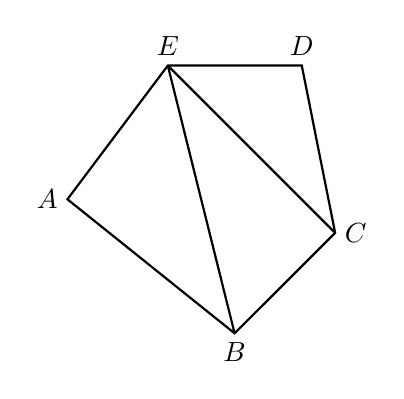
\begin{tikzpicture}
                \coordinate (A) at (0, 1.702125);
                \coordinate (B) at (2.122875, 0);
                \coordinate (C) at (3.4, 1.275);
                \coordinate (D) at (2.976125, 3.4);
                \coordinate (E) at (1.275, 3.4);

                \draw[thick] (A) -- (B) -- (C) -- (D) -- (E) -- cycle;
                \draw[thick] (B) -- (E);
                \draw[thick] (C) -- (E);

                \tikzhalflengtharrow{[xshift=-4.4625pt]B}{[xshift=-4.4625pt]E}
                \tikzhalflengtharrow{[xshift=4.4625pt]E}{[xshift=4.4625pt]B}
                \tikzhalflengtharrow{[yshift=-7.14pt]E}{[yshift=-7.14pt]A}
                \tikzhalflengtharrow{[yshift=7.14pt]B}{[yshift=7.14pt]C}
                \tikzhalflengtharrow{[yshift=6.05625pt]A}{[yshift=6.05625pt]B}
                \tikzhalflengtharrow{[yshift=-5.9925pt]C}{[yshift=-5.9925pt]E}
                \tikzhalflengtharrow{[xshift=5.9925pt]E}{[xshift=5.9925pt]C}
                \tikzhalflengtharrow{[yshift=-4.4625pt]D}{[yshift=-4.4625pt]E}
                \tikzhalflengtharrow{[xshift=-4.55175pt]C}{[xshift=-4.55175pt]D}

                \node[anchor=east] at (A) {\(A\)};
                \node[anchor=north] at (B) {\(B\)};
                \node[anchor=west] at (C) {\(C\)};
                \node[anchor=south] at (D) {\(D\)};
                \node[anchor=south] at (E) {\(E\)};
            \end{tikzpicture}
            \caption{Closed triangulated polygonal chain}\label{fig:cauchyintegraltheoremoversimplyconnectedset_closedpolygonalchaintriangulation}
        \end{minipage}
        \hfill
        \begin{minipage}{0.48\textwidth}
            \centering
            \vspace{0pt}
            \begin{tikzpicture}
                \coordinate (A) at (0, 0);
                \coordinate (D) at (4.14375, 1.59375);
                \coordinate (F) at (1.59375, 1.59375);
                \coordinate (C) at (5.1, 0);
                \coordinate (B) at (3.1875, 3.1875);
                \coordinate (E) at (2.55, 0);

                \draw[thick] (A) -- (F) -- (E) -- cycle;
                \draw[thick] (B) -- (D) -- (F) -- cycle;
                \draw[thick] (C) -- (D) -- (E) -- cycle;

                \tikzhalflengtharrow{[yshift=-7.45875pt]F}{[shift={(12.75pt,5.2275pt)}]A}
                \tikzhalflengtharrow{[yshift=-7.45875pt]B}{[shift={(12.75pt,5.2275pt)}]F}
                \tikzhalflengtharrow{[yshift=-7.45875pt]D}{[shift={(12.75pt,5.2275pt)}]E}
                \tikzhalflengtharrow{[yshift=7.45875pt]E}{[shift={(-12.75pt,-5.2275pt)}]D}

                \tikzhalflengtharrow{[shift={(-2.811375pt,-4.8705pt)}]E}{[shift={(-2.811375pt,-4.8705pt)}]F}
                \tikzhalflengtharrow{[shift={(-2.811375pt,-4.8705pt)}]D}{[shift={(-2.811375pt,-4.8705pt)}]B}
                \tikzhalflengtharrow{[shift={(-2.811375pt,-4.8705pt)}]C}{[shift={(-2.811375pt,-4.8705pt)}]D}
                \tikzhalflengtharrow{[shift={(2.811375pt,4.8705pt)}]F}{[shift={(2.811375pt,4.8705pt)}]E}

                \tikzhalflengtharrow{[yshift=4.8705pt]A}{[yshift=4.8705pt]E}
                \tikzhalflengtharrow{[yshift=4.8705pt]E}{[yshift=4.8705pt]C}
                \tikzhalflengtharrow{[yshift=4.8705pt]F}{[yshift=4.8705pt]D}
                \tikzhalflengtharrow{[yshift=-4.8705pt]D}{[yshift=-4.8705pt]F}

                \coordinate (AE) at ($(A)!0.5!(E)$);
                \coordinate (AF) at ($(A)!0.5!(F)$);
                \coordinate (FD) at ($(F)!0.5!(D)$);
                \coordinate (BF) at ($(B)!0.5!(F)$);
                \coordinate (EC) at ($(E)!0.5!(C)$);

                \path let
                \p1 = (FD),
                \p2 = (BF),
                \p3 = (AE),
                \p4 = (AF),
                \p5 = (EC)
                in
                node[shift={(3.1875pt,-3.1875pt)}] at (\x1, \y2) {\(\Delta_1\)}
                node[shift={(3.1875pt,-3.1875pt)}] at (\x3, \y4) {\(\Delta_2\)}
                node[shift={(3.1875pt,-3.1875pt)}] at (\x5, \y4) {\(\Delta_3\)}
                node[shift={(-3.1875pt, 3.1875pt)}] at (\x1, \y4) {\(\Delta_4\)};
            \end{tikzpicture}
            \caption{Quadrisection of \(\operatorname{int}\Delta\)}\label{fig:cauchyintegraltheoremoversimplyconnectedset_trianglequadrisection}
        \end{minipage}
    \end{figure}Since \(P\) is a closed polygonal chain, we can triangulate the interior. For example, consider \cref{fig:cauchyintegraltheoremoversimplyconnectedset_closedpolygonalchaintriangulation}. Then,
    \begin{align*}
        \int_{ABCDE}f(z)\ddz & =\qty(\int_{\overrightarrow{AB}}+\int_{\overrightarrow{BC}}+\int_{\overrightarrow{CD}}+\int_{\overrightarrow{DE}}+\int_{\overrightarrow{EA}})f(z)\ddz \\
        & \quad+\qty(\int_{\overrightarrow{BE}}+\int_{\overrightarrow{EB}}+\int_{\overrightarrow{CE}}+\int_{\overrightarrow{EC}})f(z)\ddz                       \\
        & =\int_{\Delta{ABE}}f(z)\ddz+\int_{\Delta{BCE}}f(z)\ddz+\int_{\Delta{CDE}}f(z)\ddz.
    \end{align*} Thus, if the integral over every triangle in \(U\) vanishes, then \cref{eq:cauchyintegraltheoremoversimplyconnectedset_statement} follows. Consider a triangle in \(U\) with boundary \(\Delta\). Then define \(M\) to be \[M=\abs{\int_{\Delta}f(z)\ddz}.\]
    We can quadrisect the triangle bounded by \(\Delta\) into four triangles with boundaries \(\Delta_1,\Delta_2,\Delta_3,\Delta_4\) as in \cref{fig:cauchyintegraltheoremoversimplyconnectedset_trianglequadrisection}. Then one of \(\Delta_1\), \(\Delta_2\), \(\Delta_3\), or \(\Delta_4\) (denote this to be \(\Delta^1\)) satisfy
    \[\abs{\int_{\Delta^1}f(z)\ddz}\geq\frac{M}{4},\]
    and recursively, choose
    \begin{equation}
        \abs{\int_{\Delta^2}f(z)\ddz}\geq\frac{M}{4^2},\ldots,\abs{\int_{\Delta^n}f(z)\ddz}\geq\frac{M}{4^n}. \label{eq:cauchyintegraltheoremoversimplyconnectedset_trianglelowerbound}
    \end{equation}
    Let \(L\) denote the perimeter of \(\Delta\). Then, the perimeters of \(\Delta^1,\Delta^2,\ldots\) respectively are \(\frac{L}{2},\frac{L}{2^2},\ldots\). As \(n\to\infty\), \(\Delta_n\) shrinks to a single point \(z_0\). Then, \(\forall n\in\mathbb{N}\), \(z_0\in\Delta^n\).

    By the definition of holomorphy, \(\forall\varepsilon>0\), \(\exists\delta>0\) such that \(\forall z\in D\paren{z_0,\delta}\), \[\abs{\frac{f\paren{z}-f\paren{z_0}}{z-z_0}-f'\paren{z_0}}<\varepsilon,\]\[\abs{f\paren{z}-f\paren{z_0}-f'\paren{z_0}\paren{z-z_0}}<\varepsilon\abs{z-z_0},\] and \(\exists N\in\mathbb{N}\) such that \(\forall n\in\mathbb{N}_{>N}\), \(\Delta^n\subset D\paren{z_0,\delta}\). By \cref{thm:cauchyintegraltheorem}, since the functions \(z\mapsto 1\) and \(z\mapsto z\) are both entire, \[\int_{\Delta^n}\ddz=0,\quad\int_{\Delta^n}z\ddz=0.\] Then
    \begin{align*}
        \int_{\Delta^n}f(z)\ddz & =\int_{\Delta^n}f(z)\ddz-f\paren{z_0}\int_{\Delta^n}\ddz-f'\paren{z_0}\qty(\int_{\Delta^n}z\ddz-z_0\int_{\Delta^n}\ddz) \\
        & =\int_{\Delta^n}\brackets{f(z)-f\paren{z_0}-f'\paren{z_0}\paren{z-z_0}}\ddz.
    \end{align*}
    Because the distance between any two points in the interior of a triangle is always less than its perimeter, using the triangle inequality for complex integrals, \[\int_{\Delta^n}\abs{f(z)}\abs{\ddz}\leq\varepsilon\int_{\Delta^n}\abs{z-z_0}\abs{\ddz}=\frac{\varepsilon L}{2^n}\int_{\Delta^n}\abs{\ddz}=\frac{\varepsilon L^2}{4^n}.\]
    Comparing the above equation with \cref{eq:cauchyintegraltheoremoversimplyconnectedset_trianglelowerbound}, \[\frac{M}{4^n}<\frac{\varepsilon L}{4^n},\quad M<\varepsilon L.\] Since \(\Delta\) is rectifiable, \(L\) is finite, and letting \(\varepsilon\to0\), we find that \(M\to0\). Then, for every triangle in \(U\), the integral vanishes, and \cref{eq:cauchyintegraltheoremoversimplyconnectedset_chainvanishingstatement,eq:cauchyintegraltheoremoversimplyconnectedset_chaindefinition} follow.
\end{proof}
\begin{theorem}[\textsc{Cauchy--Goursat}]\label{thm:cauchygoursattheorem}
    Let \(U\subset\mathbb{C}\) be an open region bounded with boundary \(\partial U\). Let \(f:U\to\mathbb{C}\) be a holomorphic function continuous on \(\overline{U}\). Then, \[\oint_{\partial U}f(\zeta)\ddzeta=0.\]
\end{theorem}
\begin{proof}
    Since \(\partial U\cap U=\varnothing\) and \(f(z)\) is not necessarily holomorphic over \(\overline{U}\), we cannot directly apply \cref{lem:cauchyintegraltheoremoversimplyconnectedset}.
    \begin{figure}
        \centering
        \begin{tikzpicture}[>=stealth,
                arrow style/.style={
                    postaction={decorate},
                    decoration={markings, mark=at position 0.5 with {\arrow[scale=1]{Stealth}}}
            }]
            \pgfmathsetmacro{\lengtheta}{18pt}
            \pgfmathsetmacro{\lengthepsilon}{20pt}
            \coordinate (M) at (1, 1.5);
            \coordinate (P) at (1, 4.2);
            \coordinate (Q) at (5, 4.4);
            \coordinate (N) at (5, 1.7);
            \coordinate (Mprime) at ([yshift=\lengtheta] M);
            \coordinate (Pprime) at ([yshift=-\lengtheta] P);
            \coordinate (Qprime) at ([yshift=-\lengtheta] Q);
            \coordinate (Nprime) at ([yshift=\lengtheta] N);
            \draw[-{Stealth}, thick] (-0.5, 0) -- (6, 0);
            \draw[-{Stealth}, thick] (0, -0.5) -- (0, 6);
            \draw[thick, arrow style] (P) -- (M);
            \draw[thick, arrow style, name path=curveQP] (Q) to[out angle=90, in angle=90, curve through = {([shift={(2, 0)}] P) ([shift={(1.5, 0.2)}] P)}] (P);
            \draw[thick, arrow style] (N) -- (Q);
            \draw[thick, arrow style, name path=curveMN] (M) to[out angle=270, in angle=270, curve through = {([shift={(-2, 0)}] N) ([shift={(-1.5, -0.2)}] N)}] (N);
            \path let \p1 = (P) in coordinate (P1x) at ({\x1 + \lengthepsilon}, 0);
            \path let \p1 = (Q) in coordinate (Q1x) at ({\x1 - \lengthepsilon}, 0);
            \path[name path=verticalleftmarker](P1x) -- (P1x |- 0, 6);
            \path[name path=verticalrightmarker](Q1x) -- (Q1x |- 0, 6);
            \path[name intersections={of=curveQP and verticalleftmarker, by=P1}];
            \path[name intersections={of=curveMN and verticalleftmarker, by=M1}];
            \draw[thin] (M1) -- (P1);
            \path[name intersections={of=curveQP and verticalrightmarker, by=Q1}];
            \path[name intersections={of=curveMN and verticalrightmarker, by=N1}];
            \draw[thin] (N1) -- (Q1);
            \draw[thin] (Mprime) to[out angle=270, in angle=270, curve through = {([shift={(-2, 0)}] Nprime) ([shift={(-1.5, -0.2)}] Nprime)}] (Nprime);
            \draw[thin] (Qprime) to[out angle=90, in angle=90, curve through = {([shift={(2, 0)}] Pprime) ([shift={(1.5, 0.2)}] Pprime)}] (Pprime);
            \draw[dashed] (M) -- (M |- 0, 0);
            \draw[dashed] (N) -- (N |- 0, 0);
            \draw[dashed] (M1) -- (P1x);
            \draw[dashed] (N1) -- (Q1x);
            \node[anchor=north east] at (M) {\(M\)};
            \node[anchor=south east] at (P) {\(P\)};
            \node[anchor=south west] at (Q) {\(Q\)};
            \node[anchor=north west] at (N) {\(N\)};
            \node[anchor=north east] at (Mprime) {\(M'\)};
            \node[anchor=south east] at (Pprime) {\(P'\)};
            \node[anchor=south west] at (Qprime) {\(Q'\)};
            \node[anchor=north west] at (Nprime) {\(N'\)};
            \node[anchor=north west] at (M1) {\(M_1\)};
            \node[anchor=south] at (P1) {\(P_1\)};
            \node[anchor=south] at (Q1) {\(Q_1\)};
            \node[anchor=north east] at (N1) {\(N_1\)};
            \node[anchor=south west] at ([yshift=\lengtheta+7pt] M1) {\(M'_1\)};
            \node[anchor=north west] at ([yshift=-\lengtheta-3pt] P1) {\(P'_1\)};
            \node[anchor=north east] at ([yshift=-\lengtheta-7pt] Q1) {\(Q'_1\)};
            \node[anchor=south east] at ([yshift=\lengtheta+3pt] N1) {\(N'_1\)};
            \node[anchor=north] at (M |- 0, 0) {\(a\)};
            \node[anchor=north] at (N |- 0, 0) {\(b\)};
            \node[anchor=north] at (P1x |- 0, 0) {\(a+\varepsilon\)};
            \node[anchor=north] at (Q1x |- 0, 0) {\(b-\varepsilon\)};
            \node[anchor=north, xshift=-2pt] at (6, 0) {\(x\)};
            \node[anchor=east, yshift=-2pt] at (0, 6) {\(y\)};
        \end{tikzpicture}
        \caption{A simplified region containing two vertical lines and two continuous, rectifiable curves.}
        \label{fig:cauchygoursattheorem_simplifiedregion}
    \end{figure}

    First assume \(U\) has the shape of \(MNQP\) in \cref{fig:cauchygoursattheorem_simplifiedregion}. That is, \(U\) consists of \(x=a\), \(x=b\) for \(a<b\), and two rectifiable \(C^0\) curves \(\overrightarrow{MN}:y=\varphi(x)\) and \(\overrightarrow{QP}:\psi(x)\) such that \(\varphi(x)<\psi(x)\), \(\forall a\le x\le b\).

    For some \(\varepsilon>0\), \(\eta>0\), construct a new curve \(M_1'N_1'Q_1'P_1'\in U\) to be the boundary of the region bounded by \(P_1M_1:x=a+\varepsilon\), \(N_1Q_1:b-\varepsilon\), \(M'N':\varphi(x)+\eta\), and \(Q'P':\psi(x)-\eta\) such that \(M_1'N_1'Q_1'P_1'\) remains simple. By \cref{lem:cauchyintegraltheoremoversimplyconnectedset}, \[\oint_{M_1'N_1'Q_1'P_1'}f(z)\ddz=0.\]
    By \cref{thm:heinecantor}, \(f(z)\) is uniformly continuous over \(\overline{U}\), and therefore \(\forall\varepsilon'>0\), we can choose \(\eta>0\) so that \(\forall z\in\overrightarrow{M_1'N_1'}\), \(\abs{f\paren{z}-f\paren{z-\eta}}<\varepsilon'\) is satisfied. Letting \(\eta\to0\) (with \(\varepsilon'\to0\)) and fixing \(\varepsilon>0\), we get that
    \begin{align*}
        \abs{\int_{\overrightarrow{M_1'N_1'}}f(z)\ddz-\int_{\overrightarrow{M_1N_1}}f(z)\ddz} & \leq\int_{\overrightarrow{M_1'N_1'}}\abs{f(z)-f\paren{z-\eta}}\abs{\ddz} \\
        & <\varepsilon'\int_{\overrightarrow{M_1'N_1'}}\abs{dz}\to0,
    \end{align*}
    and consequently,
    \begin{equation}
        \int_{\overrightarrow{M_1'N_1'}}f(z)\ddz\to\int_{\overrightarrow{M_1N_1}}f(z)\ddz.\label{eq:cauchygoursattheorem_innerinnerhorizontaltoouterinnerhorizontal1}
    \end{equation}
    Under the same limit, we get
    \begin{equation}
        \int_{\overrightarrow{Q_1'P_1'}}f(z)\ddz\to\int_{\overrightarrow{Q_1P_1}}f(z)\ddz.\label{eq:cauchygoursattheorem_innerinnerhorizontaltoouterinnerhorizontal2}
    \end{equation} By the continuity of \(f(z)\) over a compact set,
    \begin{equation}
        \int_{\overrightarrow{P_1'M_1'}}f(z)\ddz\to\int_{\overrightarrow{P_1M_1}}f(z)\ddz,\quad\int_{\overrightarrow{N_1'Q_1'}}f(z)\ddz\to\int_{\overrightarrow{N_1Q_1}}f(z)\ddz.\label{eq:cauchygoursattheorem_innerinnerverticaltoouterinnervertical}
    \end{equation}
    Then letting \(\varepsilon\to0\), for the same reason as \cref{eq:cauchygoursattheorem_innerinnerverticaltoouterinnervertical}, \cref{eq:cauchygoursattheorem_innerinnerhorizontaltoouterinnerhorizontal1,eq:cauchygoursattheorem_innerinnerhorizontaltoouterinnerhorizontal2} yield \[\int_{\overrightarrow{M_1N_1}}f(z)\ddz\to\int_{\overrightarrow{MN}}f(z)\ddz,\quad\int_{\overrightarrow{Q_1P_1}}f(z)\ddz\to\int_{\overrightarrow{QP}}f(z)\ddz.\]
    We are left to show the subsequent limits of the results from \cref{eq:cauchygoursattheorem_innerinnerverticaltoouterinnervertical}. For the left integral, let \(y_{\varphi}=\max\cbraces{\varphi(a),\varphi\paren{a+\varepsilon}}\) and \(y_{\psi}=\max\cbraces{\psi(a),\psi\paren{a+\varepsilon}}\).

    Then, \[\int_{\overrightarrow{PM}}f(z)\ddz=\ii\int_{\psi(a)}^{\varphi(a)}f\paren{a+\ii y}\ddy=\ii\paren{\int_{\psi(a)}^{y_\varphi}+\int_{y_\varphi}^{y_\psi}+\int_{y_\psi}^{\varphi(a)}}f(a+\ii y)\ddy.\]
    Similarly, \[\int_{\overrightarrow{P_1M_1}}f(z)\ddz=\ii\paren{\int_{\psi(a+\varepsilon)}^{y_\varphi}+\int_{y_\varphi}^{y_\psi}+\int_{y_\psi}^{\varphi(a+\varepsilon)}}f(a+\varepsilon+\ii y)\ddy.\]
    The difference \(\paren{\int_{\overrightarrow{PM}}-\int_{\overrightarrow{P_1M_1}}}f(z)\ddz\) between the two is then equal to
    \begin{gather*}
        \ii\int_{y_{\varphi}}^{y_{\psi}}\paren{f\paren{a+\ii y}-f\paren{a+\varepsilon+\ii y}}\ddz\\
        {}+{\ii\paren{\int_{\psi(a)}^{y_\varphi}+\int_{y_\psi}^{\varphi(a)}}f(a+\ii y)-\ii\paren{\int_{\psi(a+\varepsilon)}^{y_\varphi}z+\int_{y_\psi}^{\varphi\paren{a+\varepsilon}}}f(a+\varepsilon+\ii y)}.
    \end{gather*}
    The first term vanishes by uniform continuity (through the same argument used for \(M_1'N_1'\to M_1N_1\)) and the remaining four integrals all equal 0 as they are all integrable on a degenerating interval (as \(\varepsilon\to0\), \(y_\varphi\to\varphi(a)\) and \(y_\psi\to\psi(a)\) because \(\varphi,\psi\in C^0\)). Therefore, \[\int_{\overrightarrow{P_1M_1}}f(z)\ddz\to\int_{\overrightarrow{PM}}f(z)\ddz,\]
    and through similar logic, \[\int_{\overrightarrow{N_1Q_1}}f(z)\ddz\to\int_{\overrightarrow{NQ}}f(z)\ddz.\] Therefore, \[\oint_{MNQP}f(z)\ddz=0.\]
    Any open region \(U\subset\mathbb{C}\) with a simple closed boundary can be broken up into smaller regions with the same form as \(MNQP\) with finitely many auxiliary lines. Then the conclusion follows.
\end{proof}
\begin{remark}
    The theorem is also valid for any multiply connected region (and its boundary will consist of multiple curves) as a multiply connected region is equal to the union of several simply connected regions with vertical auxiliary lines between.

    Additionally, if \(U\subset\mathbb{C}\) is simply connected and \(f\) is holomorphic on \(U\), then for any two points \(z,z_0\in U\), the integral \[\int_{z_0}^z f(\zeta)\ddzeta\] is well-defined and independent of the path taken from \(z_0\) to \(z\). In this sense, a holomorphic function behaves analogously to a potential field.
\end{remark}
\begin{theorem}[\textsc{Cauchy--Goursat}]\label{thm:cauchygoursatformula}
    Let \(U\subset\mathbb{C}\) be an open region bounded with a simple closed boundary \(\partial U\), and let \(f:U\to\mathbb{C}\) be a holomorphic function continuous on \(\overline{U}\). Then for all \(z\in U\),
    \begin{equation}
        f(z)=\frac{1}{2\uppi\ii}\oint_{\partial U}\frac{f(\zeta)}{\zeta-z}\ddzeta.\label{eq:cauchygoursatformula}
    \end{equation}
\end{theorem}
\begin{proof}
    By the Cauchy--Goursat Theorem (\cref{thm:cauchygoursattheorem}), \[\int_{\partial\paren{U\setminus D(z,\varepsilon)}}\frac{f(\zeta)}{\zeta-z}\ddzeta=\oint_{\partial U}\frac{f(\zeta)}{\zeta-z}\ddzeta-\oint_{\partial D(z,\varepsilon)}\frac{f(\zeta)}{\zeta-z}\ddzeta=0.\]
    From rearrangement, \[\oint_{\partial U}\frac{f(\zeta)}{\zeta-z}\ddzeta=2\uppi\ii f(z)+\ii\int_0^{2\uppi}\paren{f\paren{z+\varepsilon\ee^{\ii t}}-f(z)}\dd{t}.\]
    Since \(f\in C^0(\partial D(z,\varepsilon))\), as \(\varepsilon\to0\),
    \begin{align*}
        \abs{\int_0^{2\uppi}\paren{f\paren{z+\varepsilon\ee^{\ii t}}-f(z)}\dd{t}} & \leq\int_0^{2\uppi}\abs{f\paren{z+\varepsilon\ee^{\ii t}}-f(z)}\dd{t}            \\
        & \leq2\uppi\max_{t\in[0,2\uppi]}\abs{f\paren{z+\varepsilon\ee^{\ii t}}-f(z)}\to0.
    \end{align*}
    By rearrangement, \[f(z)=\frac{1}{2\uppi\ii}\oint_{\partial U}\frac{f(\zeta)}{\zeta-z}\ddzeta.\qedhere\]
\end{proof}
\begin{remark}
    In the proof of \cref{thm:pompeiu}, we used Lipschitz continuity for a smooth function, which was a stronger condition than necessary. The true necessity of smoothness was to be able to apply Green's Theorem (\cref{thm:complexgreen}).
\end{remark}
This profound theorem is extremely important and helpful in complex integration and essential in the evaluation of integrals, as demonstrated below.
\begin{example}\label{ex:cauchygoursatformulazeroofunity}
    Evaluate the integral \(\oint_{\partial D(0,2)}\frac{\ddz}{z^n-1}\), where \(n\in\mathbb{N}_{\geq 2}\).
\end{example}
\begin{proof}
    Since \(z^n-1=\prod_{k=0}^{n-1}\qty(z-\omega^k_n)\), where \(\omega^k_n=\ee^{\ii\uppi\frac{k}{n}}\), the integrand has singularities at every \(n\)-th zero of unity. Then the integral is equal to:
    \begin{equation}
        \oint_{\partial D(0,2)}\frac{\ddz}{\prod_{j=0}^{n-1}\qty(z-\omega_j)}=\oint_{\partial D(0,2)}\sum_{j=0}^{n-1}\frac{c_j}{z-\omega_j}\ddz,\label{eq:cauchygoursatformulazerosofunity}
    \end{equation}
    where \(\cbraces{c_j}\) are the coefficients of the partial fraction decomposition. By the Cauchy--Goursat Formula (\cref{thm:cauchygoursatformula}), \cref{eq:cauchygoursatformulazerosofunity} becomes: \[\sum_{k=0}^{n-1}\oint_{\partial D(0,2)}\frac{c_k}{z-\omega_k}\ddz=2\uppi\ii\sum_{k=0}^{n-1}c_k.\]
    Observe that \(\sum_{k=0}^{n-1} c_k=\lim_{z\to\infty}\sum_{k=0}^{n-1}\frac{zc_k}{z-\omega_k}=\lim_{z\to\infty}\frac{z}{z^n-1}=0\) since \(n\geq2\). Therefore, \[\oint_{\partial D(0,2)}\frac{\ddz}{z^n-1}=0.\qedhere\]
\end{proof}
We have also already seen the utility of parameterization via a polar transformation. Many useful identities in classical calculus can also be derived from concepts in its generalization:
\begin{example}
    Prove that \(\forall n\in\mathbb{N}\), \[\int_{0}^{2\uppi}\cos^{2n}\theta\dd{\theta}=2\uppi\prod_{k=1}^n\frac{2k-1}{2k}.\]
\end{example}
\begin{proof}
    Consider the integral \[\oint_{\partial\mathbb{D}}\qty(z+\frac{1}{z})^{2n}\frac{\ddz}{z}.\]
    Letting \(z=\ee^{\ii\theta}\), we get \(\oint_{\partial\mathbb{D}}\qty(\ee^{\ii\theta}+\ee^{-\ii\theta})^{2n}\ee^{-\ii\theta}\ddz=2^{2n}\ii\int_0^{2\uppi}\cos^{2n}\theta\dd{\theta}\). Alternatively, we can expand the integrand and get \[\oint_{\partial\mathbb{D}}\sum_{k=0}^{2n}\binom{2n}{k}z^{2k-2n}\frac{\ddz}{z}=\sum_{k=0}^{2n}\oint_{\partial\mathbb{D}}\binom{2n}{k}z^{2k-2n-1}\ddz.\]
    When \(2k-2n-1\ge0\), the integrand is holomorphic. The integral is then equal to \[\binom{2n}{0}\oint_{\partial\mathbb{D}}z^{-2n-1}\ddz+\binom{2n}{1}\oint_{\partial\mathbb{D}}z^{-2n+1}\ddz+\cdots+\binom{2n}{n}\oint_{\partial\mathbb{D}}\frac{\ddz}{z}=2\uppi\ii\binom{2n}{n},\]
    since all the higher order terms vanish:
    \[\oint_{\partial\mathbb{D}}z^{2k-2n-1}\ddz=\ii\int_0^{2\uppi}\ee^{2\ii\theta(k-n)}\dd{\theta}=
        \begin{dcases}
            0         & \qif* k<n, \\
            2\uppi\ii & \qif* k=n.
    \end{dcases}\]
    Therefore, \[2^{2n}\ii\int_0^{2\uppi}\cos^{2n}\theta\dd{\theta}=2\uppi\ii\binom{2n}{n}\Longleftrightarrow\int_0^{2\uppi}\cos^{2n}\theta\dd{\theta}=\frac{2\uppi\qty(2n)!}{2^{2n}\qty(n!)^2}=\frac{2\uppi\prod_{k=1}^{2n}k}{\prod_{k=1}^{n}{\qty(2k)}^2}.\]
    From simple cancellation, we get \[2\uppi\frac{\prod_{k=1}^{n}\qty(2k-1)}{\prod_{k=1}^n\qty(2k)}=2\uppi\prod_{k=1}^n\frac{2k-1}{2k},\]
    as expected.
\end{proof}
\begin{example}[Cauchy--Goursat Formula on the Exterior]\label{ex:cauchygoursatformulaexterior}
    Let \(\gamma\subset\mathbb{C}\) be a simple closed curve, and suppose that \(f:\mathrm{ext}(\gamma)\to\mathbb{C}\) is holomorphic and continuous on \(\overline{\mathrm{ext}(\gamma)}=\mathbb{C}\setminus\mathrm{int}(\gamma)\), where \(\mathrm{int}\) and \(\mathrm{ext}\) respectively denote the interior and exterior as in \cref{thm:jordancurve}.
    \begin{enumerate}
        \item If \(f\) has a removable singularity at \(\infty\), or if \(w=\lim_{z\to\infty} f(z)\) exists and is finite, then \(\forall z\in\mathbb{C}\setminus\gamma\), \[\frac{1}{2\uppi\ii}\oint_\gamma\frac{f(\zeta)}{\zeta-z}\ddzeta=
                \begin{dcases}
                    w      & \qif* z\in\mathrm{int}(\gamma), \\
                    w-f(z) & \qif* z\in\mathrm{ext}(\gamma).
            \end{dcases}\]
        \item If \(\gamma\) encloses the origin, then \(\forall z\in\mathbb{C}\setminus\gamma\), then
            \begin{equation}
                \frac{1}{2\uppi\ii}\oint_\gamma\frac{zf(\zeta)}{z\zeta-\zeta^2}\ddzeta=
                \begin{dcases}
                    0    & \qif* z\in\mathrm{int}(\gamma),                                                       \\
                    f(z) & \qif* z\in\mathrm{ext}(\gamma).\label{eq:cauchygoursatformulaexteriorpart2_statement}
                \end{dcases}
            \end{equation}
    \end{enumerate}
\end{example}
\begin{proof}
    \begin{enumerate}
        \item By the compactness of \(\gamma\), it can be completely contained within a sufficiently large disk centered at the origin (\(\gamma\subset D(0,R)\)). Then by applying \cref{thm:cauchygoursatformula} or \cref{thm:cauchygoursattheorem} on the set \(D(0,R)\cap\mathrm{ext}(\gamma)=D(0,R)\setminus\overline{\mathrm{int}(\gamma)}\), we get that \[\frac{1}{2\uppi\ii}\oint_{\partial D(0,R)}\frac{f(\zeta)}{\zeta-z}\ddzeta=\frac{1}{2\uppi\ii}\oint_\gamma\frac{f(\zeta)}{\zeta-z}\ddzeta+
                \begin{dcases}
                    0    & \qif* z\in\mathrm{int}(\gamma),            \\
                    f(z) & \qif* z\in D(0,R)\cap\mathrm{ext}(\gamma).
            \end{dcases}\]
            By letting \(R\to\infty\) and letting \(\zeta=R\ee^{\ii\theta}\), we get that \[\frac{1}{2\uppi\ii}\oint_\gamma\frac{f(\zeta)}{\zeta-z}\ddzeta=\frac{1}{2\uppi}\lim_{R\to\infty}\int_0^{2\uppi}\frac{f\qty(R\ee^{\ii\theta})}{1-\frac{z}{R\ee^{\ii\theta}}}\dd{\theta}-
                \begin{dcases}
                    0    & \qif* z\in\mathrm{int}(\gamma), \\
                    f(z) & \qif* z\in\mathrm{ext}(\gamma).
            \end{dcases}\]
            By the continuity of \(f\) on \(\partial D(0,R)\), it attains its maximum \(M\). For sufficiently large \(R\), \(\abs{1-\frac{z}{R\ee^{\ii\theta}}}\) attains a positive minimum. Then the integrand is uniformly bounded in \(R\) and \(\theta\), and hence the order of the limit and the integral may be exchanged. Hence,
            \begin{align*}
                \frac{1}{2\uppi\ii}\oint_\gamma\frac{f(\zeta)}{\zeta-z}\ddzeta & =\frac{1}{2\uppi}\int_0^{2\uppi}\frac{w}{1-\lim_{R\to\infty}\frac{z}{R\ee^{\ii\theta}}}\dd{\theta}-
                \begin{dcases}
                    0    & \qif* z\in\mathrm{int}(\gamma), \\
                    f(z) & \qif* z\in\mathrm{ext}(\gamma),
                \end{dcases}                                                                                                                               \\        & =
                \begin{dcases}
                    w      & \qif* z\in\mathrm{int}(\gamma), \\
                    w-f(z) & \qif* z\in\mathrm{ext}(\gamma),
                \end{dcases}
            \end{align*} as expected.
        \item Under the partial fraction decomposition of \cref{eq:cauchygoursatformulaexteriorpart2_statement}, we get that
            \begin{align}
                I & =\oint_\gamma\frac{zf(\zeta)}{z\zeta-\zeta^2}\ddzeta=\oint_\gamma\qty(\frac{f(\zeta)}{\zeta}-\frac{f(\zeta)}{\zeta-z})\ddzeta\nonumber \\
                & =\int_0^{2\uppi}\qty(f\qty(R\ee^{\ii\theta})-\frac{f\qty(R\ee^{\ii\theta})}{1-\frac{z}{R\ee^{\ii\theta}}})\dd{\theta}+
                \begin{dcases}
                    0              & \qif* z\in\mathrm{int}(\gamma),            \\
                    2\uppi\ii f(z) & \qif* z\in\mathrm{ext}(\gamma)\cap D(0,R),
                \end{dcases}\label{eq:cauchygoursatformulaexteriorpart2_prelimitintegral}
            \end{align} when \(\gamma\subset D(0,R)\).
            We will analyze the first integral as \(R\to\infty\). By the triangle and reverse triangle inequalities,
            \begin{align*}
                \qty|\int_0^{2\uppi}\qty(f\qty(R\ee^{\ii\theta})-\frac{f\qty(R\ee^{\ii\theta})}{1-\frac{z}{R\ee^{\ii\theta}}})\dd{\theta}| & \leq\int_0^{2\uppi}\qty|\frac{z}{R\ee^{\ii\theta}-z}|\dd{\theta}                             \\
                & \leq\int_0^{2\uppi}\frac{\abs{z}}{R-\abs{z}}\dd{\theta}=\frac{2\uppi\abs{z}}{R-\abs{z}}\to0.
            \end{align*}
    \end{enumerate}
    By substituting the result into \cref{eq:cauchygoursatformulaexteriorpart2_prelimitintegral}, and letting \(R\to\infty\), we get that \[\frac{1}{2\uppi\ii}\oint_\gamma\frac{zf(\zeta)}{z\zeta-\zeta^2}\ddzeta=
        \begin{dcases}
            0    & \qif* z\in\mathrm{int}(\gamma), \\
            f(z) & \qif* z\in\mathrm{ext}(\gamma),
    \end{dcases}\] as desired.
\end{proof}
